Die Leerlaufspannung $U_{\text{0}}$ bezeichnet die Spannung, die ohne
fließenden Strom $I$ an der Spannungsquelle gemessen werden kann.
Sobald ein endlicher Strom fließt, sinkt die Spannung $U_{\text{k}}$ auf einen
Wert unterhalb $U_{\text{0}}$ ab. $U_{\text{K}}$ bezeichnet hierbei die
Klemmenspannung und fällt über der Spannungsquelle ab.
Dieser Spannungsabfall lässt sich durch den Innenwiderstand der Spannungsquelle
erklären.

Gemäß dem Zweiten Kirchhoffschen Gesetz
\begin{equation}
  \sum_\symup{n} \symup{U}_{0_\symup{n}} = \symup{\sum_m R_m I_m}
  \label{eqn:kirch}
\end{equation}
ist die Summer aller Leerlaufspannungen gleich der Summe aller
Spannungsabfälle an den Widerständen $\symup{R_m}$ der Masche.
Unter Berücksichtigung von
\begin{equation}
  U=R\cdot I
\end{equation}
und Formel (\ref{eqn:kirch}) gilt für Abbildung (\ref{fig:real})
\begin{equation}
  U_\symup{0}=I \cdot R_\symup{i} + I \cdot R_\symup{a}
  \text{bzw.}
  U_\symup{k}=I \cdot R_\symup{i} = U_\symup{0} - I \cdot R_\symup{a}
  \label{eqn:U0k}
\end{equation}
\begin{figure}[H]
   \centering
  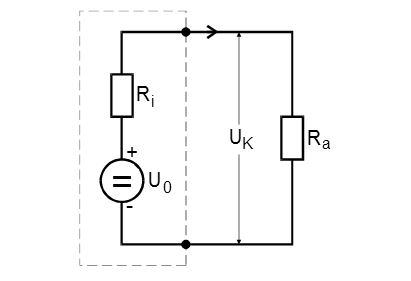
\includegraphics{bilder/real}
  \caption{Ersatzschaltbild einer realen Spannungsquelle mit Lastwiderstand
  $\symup{R_a}$ \cite{301}}
  \label{fig:real}
\end{figure}
Dabei ist $R_\symup{i}$ der Innenwiderstand der Stromquelle und $R_\symup{a}$
der Lastwiderstand im Stromkreis.
Der gestrichelt umrandete Teil von Abbildung \ref{fig:real} wird als
Ersatzschaltbild einer realen Spannungsquelle bezeichnet. Diese besteht aus
einer idealen Spannungsquelle und einem zugehörigen Innenwiderstand
$R_\symup{i}$.
Aus Formel (\ref{eqn:U0k}) wird ersichtlich, dass ein möglichst hochohmiges
Voltmeter für die Messung der Leerlaufspannung verwendet werden muss, um den
Stromfluss zu minimieren. Unter diesen Voraussetzungen gilt dann
\begin{equation*}
  I R_\symup{i} \rightarrow 0 \Rightarrow U_\symup{k} = U_\symup{0}
\end{equation*}
Da der Innenwiderstand bei anderen Spannungsquellen durch einen
Rückkopplungsmechanismus festgelegt ist, muss dieser über
\begin{equation}
  R_\symup{i}=\frac{\symup{d}U_\symup{k}}{\symup{d}I}
\end{equation}
differentiell dargestellt werden.

Die Existenz des Innenwiderstands führt dazu, dass einer Spannungsquelle keine
beliebig hohe Leistung entnommen werden kann. Für die Leistung gilt die Formel
\begin{equation}
  N=I^2R_\symup{a}
\end{equation}
als Funktion von $R_\symup{a})$. Diese Funktion erreicht ihr Maximum, wenn
\begin{equation*}
  R_\symup{a} = R_\symup{i}
\end{equation*}
gilt. Dieser Zustand wird als Leistungsanpassung bezeichnet.
